%%%%%%%%%%%%%%%%%%%%%%%%%%%%%%%%%%%%%
%                                   %
% Compile with XeLaTeX and biber    %
%                                   %
% Questions or comments:            %
%                                   %
% joshua dot mcneill at uga dot edu %
%                                   %
%%%%%%%%%%%%%%%%%%%%%%%%%%%%%%%%%%%%%

\documentclass{beamer}
  % Read in standard preamble (cosmetic stuff)
  %%%%%%%%%%%%%%%%%%%%%%%%%%%%%%%%%%%%%%%%%%%%%%%%%%%%%%%%%%%%%%%%
% This is a standard preamble used in for all slide documents. %
% It basically contains cosmetic settings.                     %
%                                                              %
% Joshua McNeill                                               %
% joshua dot mcneill at uga dot edu                            %
%%%%%%%%%%%%%%%%%%%%%%%%%%%%%%%%%%%%%%%%%%%%%%%%%%%%%%%%%%%%%%%%

% Beamer settings
% \usetheme{Berkeley}
\usetheme{CambridgeUS}
% \usecolortheme{dove}
% \usecolortheme{rose}
\usecolortheme{seagull}
\usefonttheme{professionalfonts}
\usefonttheme{serif}
\setbeamertemplate{bibliography item}{}

% Packages and settings
\usepackage{fontspec}
  \setmainfont{Charis SIL}
\usepackage{hyperref}
  \hypersetup{colorlinks=true,
              allcolors=blue}
\usepackage{graphicx}
  \graphicspath{{../../figures/}}
\usepackage[normalem]{ulem}
\usepackage{enumerate}

% Document information
\author{M. McNeill}
\title[FREN2001]{Français 2001}
\institute{\url{joshua.mcneill@uga.edu}}
\date{}

%% Custom commands
% Lexical items
\newcommand{\lexi}[1]{\textit{#1}}
% Gloss
\newcommand{\gloss}[1]{`#1'}
\newcommand{\tinygloss}[1]{{\tiny`#1'}}
% Orthographic representations
\newcommand{\orth}[1]{$\langle$#1$\rangle$}
% Utterances (pragmatics)
\newcommand{\uttr}[1]{`#1'}
% Sentences (pragmatics)
\newcommand{\sent}[1]{\textit{#1}}
% Base dir for definitions
\newcommand{\defs}{../definitions}


  % Packages and settings
  \usepackage{xcolor}
  \usepackage{listings}
    \lstset{basicstyle=\ttfamily\small,
            breaklines=true}
  \usepackage[style=apa, backend=biber]{biblatex}
    \addbibresource{../references/References.bib}

  % Document information
  \subtitle[Computational Linguistics and Corpora]{Computational Linguistics and Corpora}

  %% Custom commands
  % Subsection/frame title
  \newcommand{\suboneone}{What is it?}
  \newcommand{\subtwoone}{What are they?}
  \newcommand{\subtwotwo}{Types of corpora}

\begin{document}
  % Read in the standard intro slides (title page and table of contents)
  %%%%%%%%%%%%%%%%%%%%%%%%%%%%%%%%%%%%%%%%%%%%%%%%%%%%%%%%%%%%%%%%
% This is a standard set of intro slides used in for all slide %
% documents. It basically contains the title page and table of %
% contents.                                                    %
%                                                              %
% Joshua McNeill                                               %
% joshua dot mcneill at uga dot edu                            %
%%%%%%%%%%%%%%%%%%%%%%%%%%%%%%%%%%%%%%%%%%%%%%%%%%%%%%%%%%%%%%%%

\begin{frame}
  \titlepage
  \tiny{Office: % Basically a variable for office hours location
Gilbert 121\\
        Office hours: % Basically a variable for office hours
 lundi, mercredi, vendredi 10:10--11:10
}
\end{frame}

\begin{frame}
  \tableofcontents[hideallsubsections]
\end{frame}

\AtBeginSection[]{
  \begin{frame}
    \tableofcontents[currentsection,
                     hideallsubsections]
  \end{frame}
}


  \section{Computational Linguistics and Corpora}
    \subsection{\suboneone}
      \begin{frame}[t]{\suboneone}
        \begin{definition}
          % Computational linguistics
The study of how to engineer computers to process and produce language

          \only<1>{
            \begin{itemize}
              \item Also called \alert{natural language processing} or NLP
            \end{itemize}
          }
        \end{definition}
        \only<2>{
          \begin{block}{Two goals of this engineering}
            Basing models on linguistic theories allows us to test those theories
          \end{block}
          \lstinputlisting[firstline=3, lastline=10]{../data/grammar.py}
        }
        \only<3->{
          \begin{block}{Two goals of this engineering}
            Models allow us to interact with computers and process data more efficiently
          \end{block}
          \begin{columns}
            \column{0.5\linewidth}
              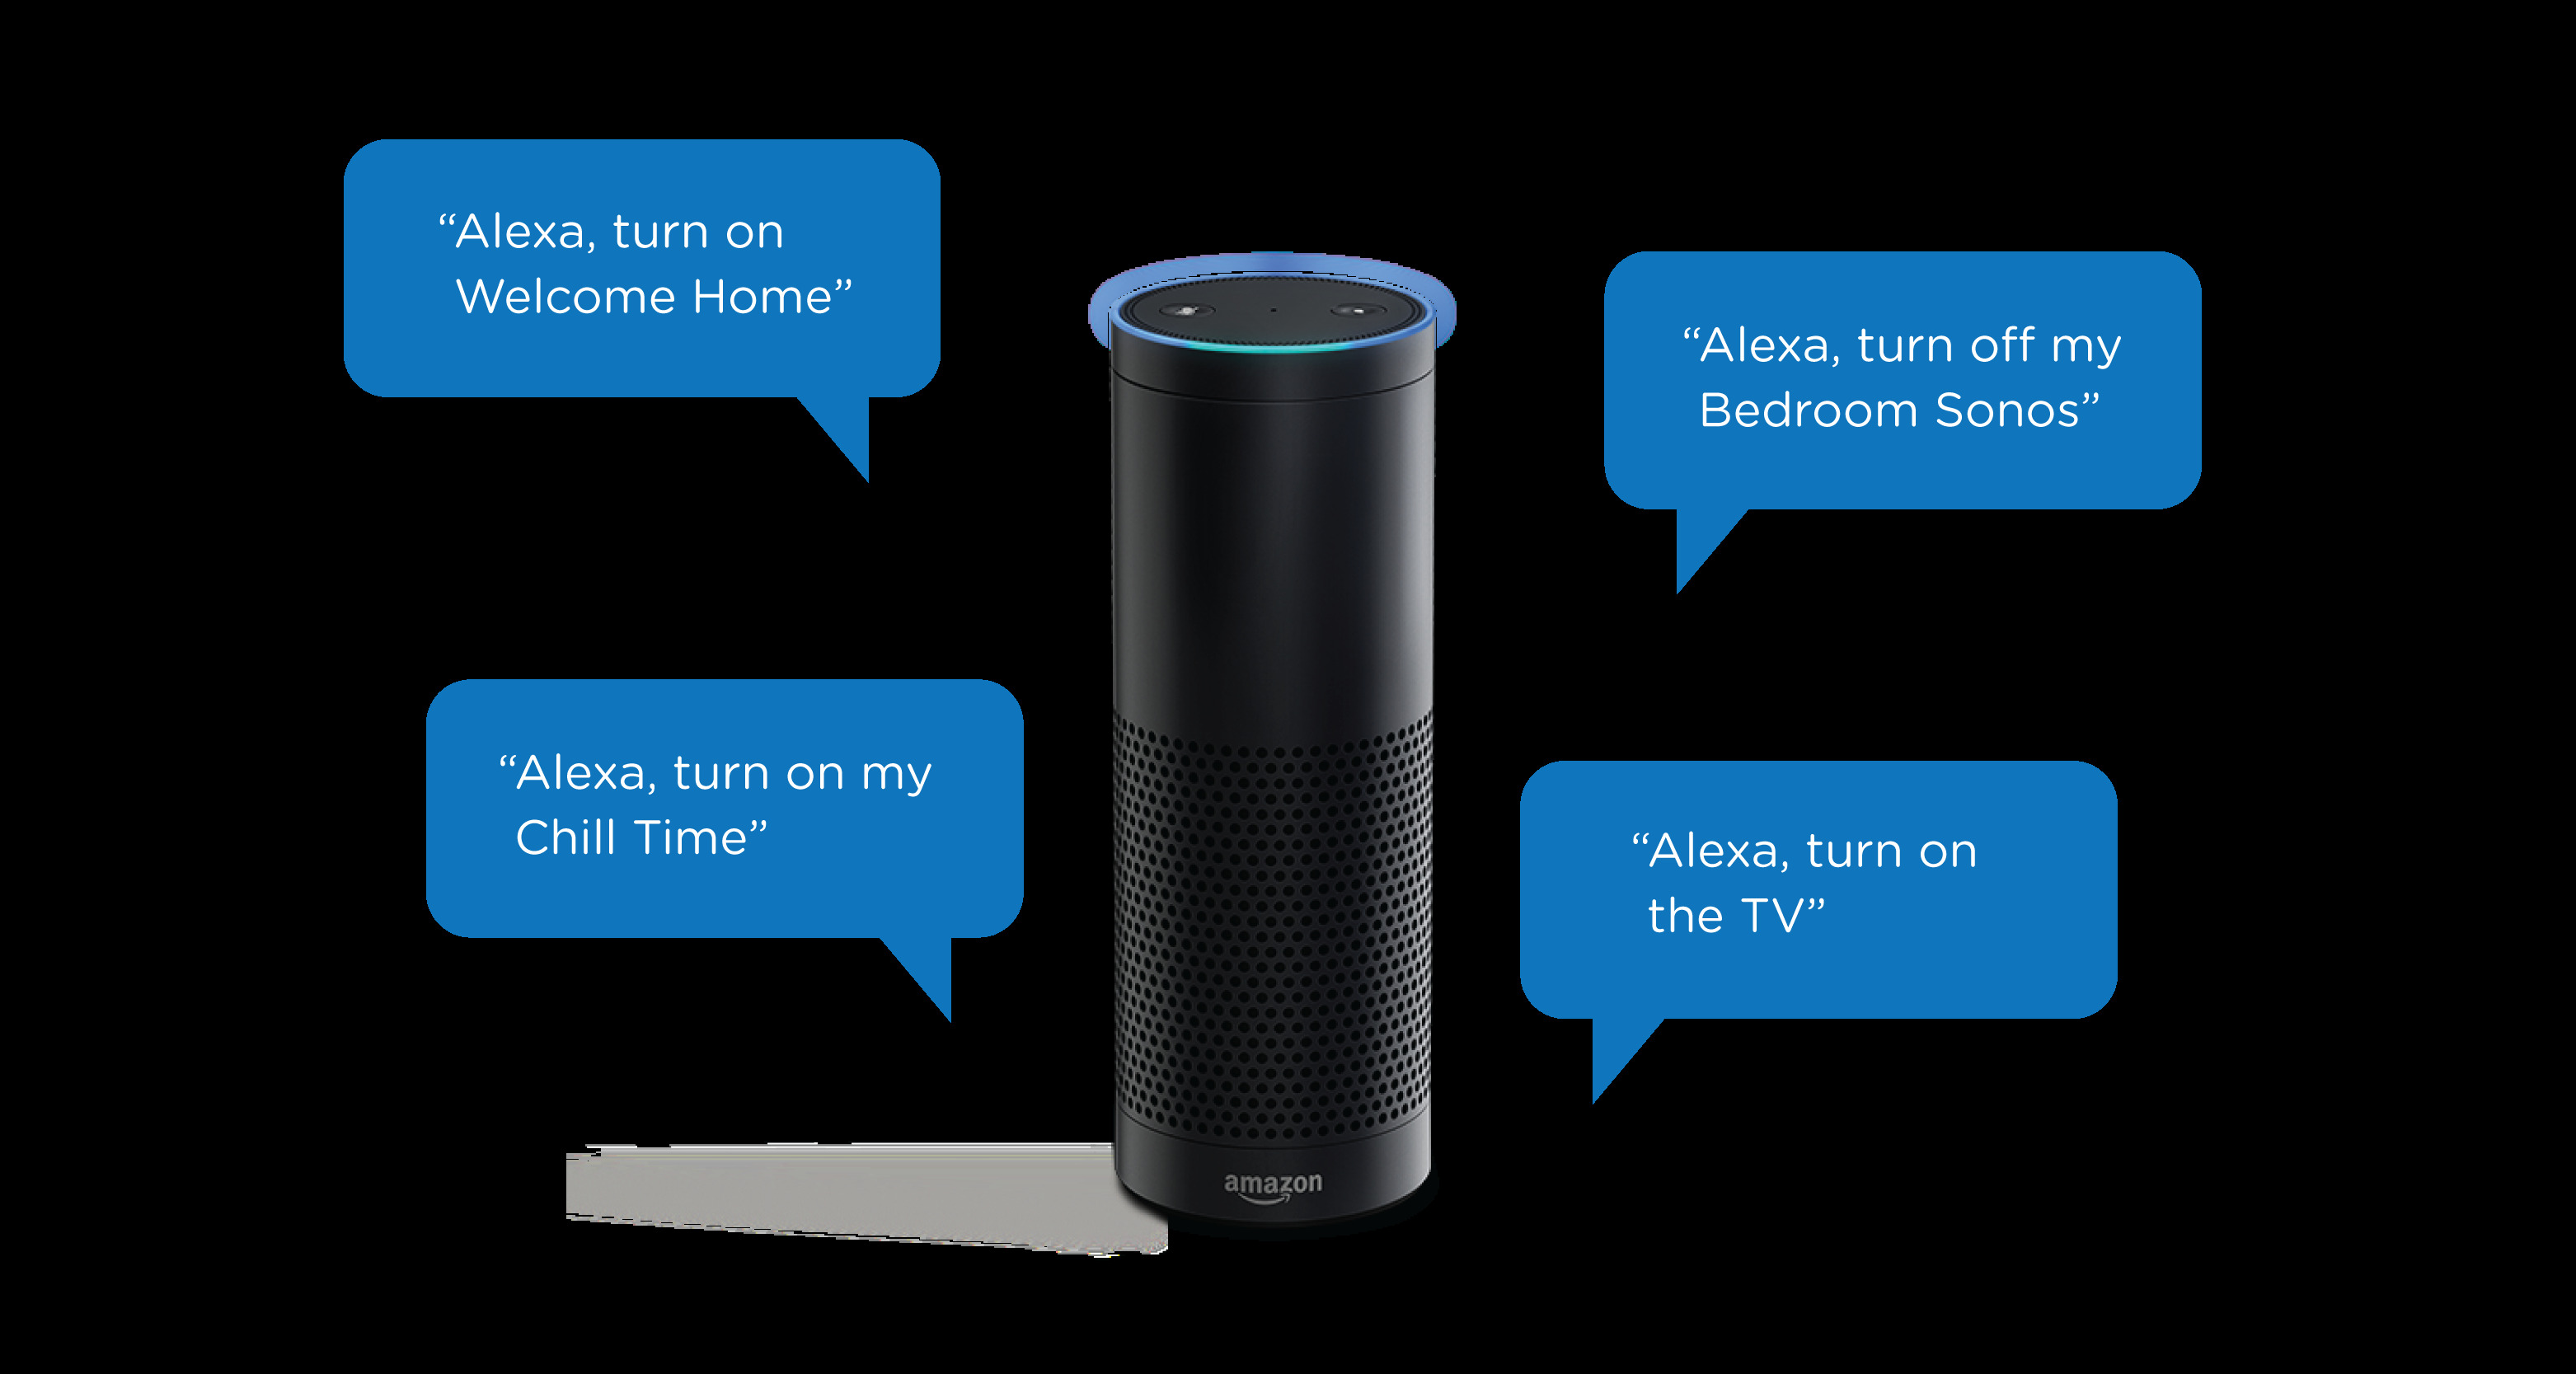
\includegraphics[scale=0.1]{alexa.jpg}
            \column{0.5\linewidth}
              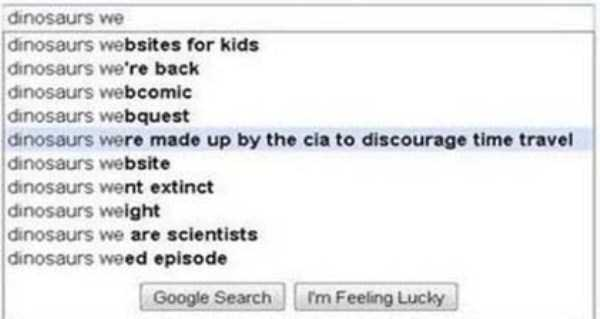
\includegraphics[scale=0.325]{autocomplete_dino.jpg}
          \end{columns}
        }
      \end{frame}

  \section{Corpora}
    \subsection{\subtwoone}
      \begin{frame}{\subtwoone}
        \begin{alertblock}{Corpus}
          % Corpus
A sample of language recorded as text, audio, or both

        \end{alertblock}
        \begin{example}
          \begin{itemize}
            \item Shakespeare's works
            \item Google Books
            \item Sociolinguistic interviews
            \item NY Times newspapers from 1987 to 2007
          \end{itemize}
        \end{example}
      \end{frame}

      \begin{frame}[t]{\subtwoone}
        \begin{block}{}
          \begin{tabular}{l r}
            \multicolumn{2}{c}{The NY Times} \\
            \hline
            Tokens                & 1,350,046,523 \\
            \uncover<3->{Annotations} & \uncover<3->{part-of-speech \& lemma}
          \end{tabular}
        \end{block}
        \only<1>{
          \begin{alertblock}{Token}
            % Token
An occurrence of a unit (usually a word) in a corpus

          \end{alertblock}
          \begin{alertblock}{Type}
            % Type
A unit (usually a word) that appears at least once in a corpus

          \end{alertblock}
        }
        \only<2>{
          \lstinputlisting[lastline=10]{../data/prep_token_type.txt}
        }
        \only<3>{
          \begin{alertblock}{Annotation}
            % Annotation
A label for a token in a corpus that provides information about that token

          \end{alertblock}
          \begin{alertblock}{Lemma}
            % Lemma
The bare, citation form of a word

            \begin{itemize}
              \item You would look up \lexi{lasers} under the lemma \lexi{laser} in the dictionary
            \end{itemize}
          \end{alertblock}
        }
        \only<4>{
          \begin{block}{Part-of-speech annotations from the Brown corpus \parencite{francis_brown_1964}}
            Here, the format is \texttt{word/pos}
            \begin{itemize}
              \item You might also find \texttt{<pos>word</pos>}
            \end{itemize}
          \end{block}
          \lstinputlisting[firstline=15, lastline=15]{../data/brown.txt}
        }
        \only<5>{
          \begin{block}{How often do all four parts of our NP rule appear with the lemma \lexi{senator}?}
            \begin{enumerate}
              \item Log on to the UGA corpus server: \url{https://research.franklin.uga.edu/linglab/corpora}
              \item Load CQP: \texttt{cqp -eC}
              \item Load the NYT corpus: \texttt{NYT;}
              \item Perform a query: \texttt{[pos="DT"] @[pos="JJ"] [lemma="senator"] [pos="IN"];}
            \end{enumerate}
          \end{block}
        }
        \only<6>{
          \begin{block}{And for fun...}
            Check which adjectives are most frequently used to describe senators
            \begin{enumerate}
              \setcounter{enumi}{4}
              \item Type: \texttt{count Last by word on target[0];}
            \end{enumerate}
          \end{block}
        }
      \end{frame}

      \begin{frame}[t]{\subtwotwo}
        \begin{block}{Other levels of annotations}
          \begin{itemize}
            \item Syntactic structure (a \alert{treebank})
            \item<3-> Phonetic transcription
            \item<4-> Compositional semantics
          \end{itemize}
        \end{block}
        \only<1>{
          \begin{columns}
            \column{0.6\linewidth}
              \lstinputlisting[basicstyle=\tiny]{../data/treebank_tree.py}
            \column{0.4\linewidth}
              \begin{block}{}
                From the Penn Treebank \parencite{marcus_building_1993}
              \end{block}
          \end{columns}
        }
        \only<2>{
          \begin{center}
            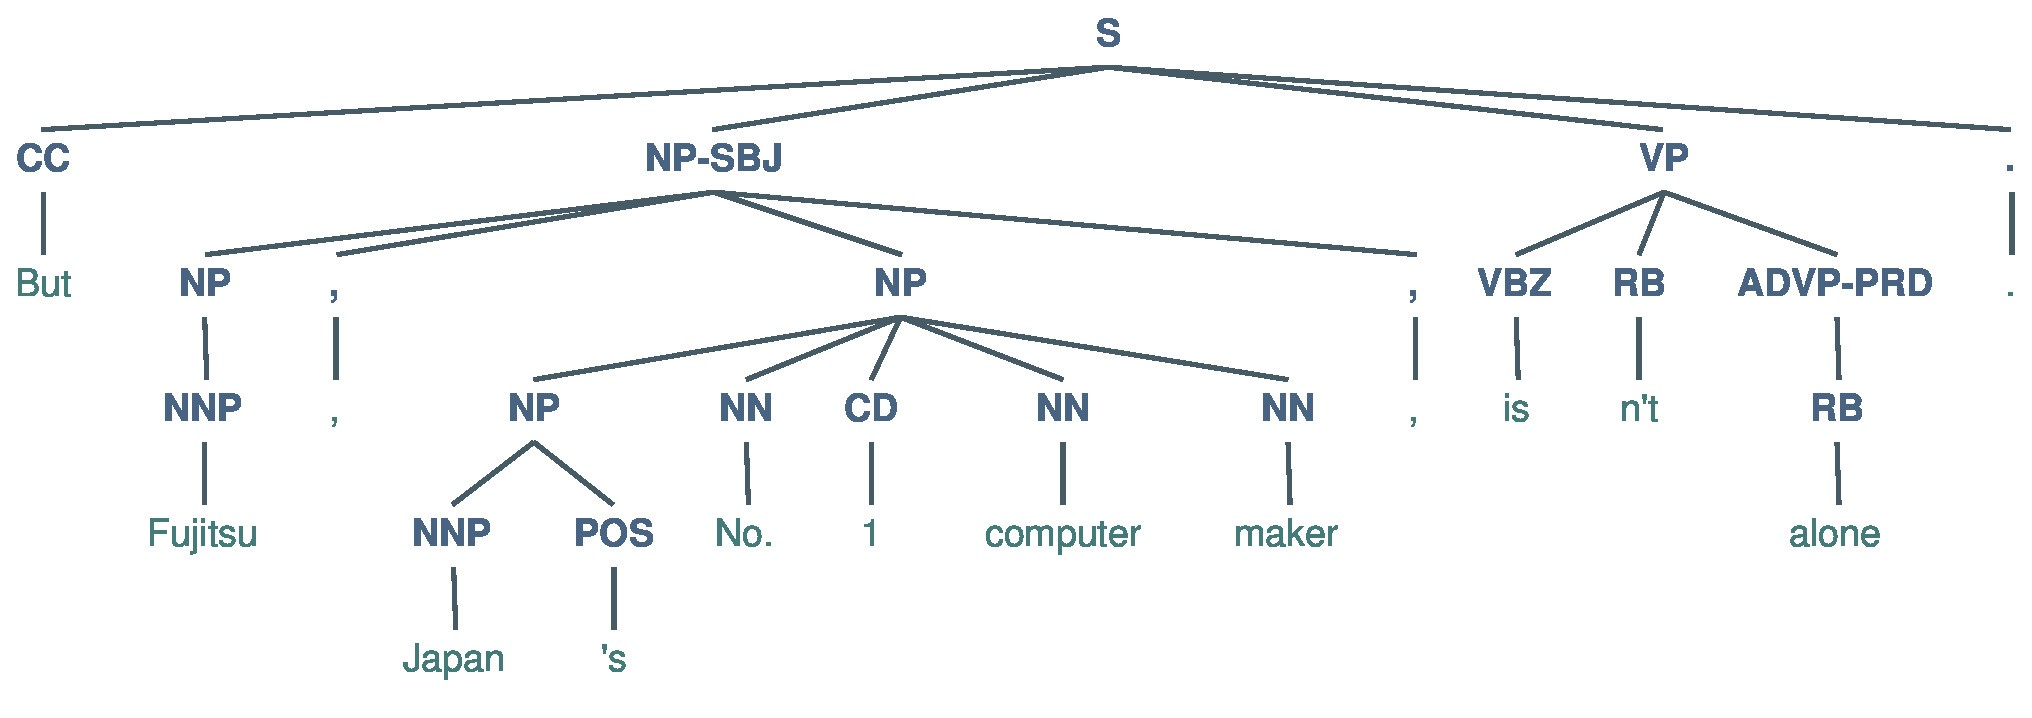
\includegraphics[scale=0.275]{treebank_examp.jpg}
          \end{center}
        }
        \only<3->{
          \begin{columns}
            \column{0.5\linewidth}
              \lstinputlisting[basicstyle=\tiny, firstline=300, lastline=315]{../data/cmudict-0.7b}
            \column{0.5\linewidth}
              \begin{block}{}
                From the CMU Pronouncing Dictionary
                \begin{itemize}
                  \item \alert{ARPAbet}: % ARPAbet
A phonetic alphabet for English made to be easily readable by computers

                \end{itemize}
              \end{block}
          \end{columns}
        }
      \end{frame}

    \subsection{\subtwotwo}
      \begin{frame}{\subtwotwo}
        \begin{block}{What variety does the NYT corpus tell us about?}
          \uncover<2->{
            One register: Journalistic writing at the NYT
          }
        \end{block}
        \begin{alertblock}<2->{Balanced corpus}
          % Balanced corpus
A corpus that

        \end{alertblock}
      \end{frame}

      \begin{frame}{\subtwotwo}
        \begin{block}{The British National Corpus (BNC) \parencite{bnc_consortium_british_2007}}
          Meant to be representative of late 20th century British English by including:
          \begin{tabular}{l l}
            \hline
            Writing             & Speech \\
            \hline
            Newspapers          & In different institutional settings \\
            Scientific articles & Private conversations \\
            Magazines           & \\
            Fiction             &
          \end{tabular}
        \end{block}
      \end{frame}

      \begin{frame}{\subtwotwo}
        \begin{block}{Corpus of Contemporary American English (COCA) \parencite{davies_corpus_2010}}
          Meant to be representative of American English since the 1990s in the same way
          \begin{itemize}
            \item A \alert{monitor corpus}: % Monitor corpus
A corpus that is continually added to over time

            \item As opposed to a \alert{reference corpus}: % Reference corpus
A corpus that is meant to be a snapshot of language in one time and place

          \end{itemize}
        \end{block}
      \end{frame}

      \begin{frame}{\subtwotwo}
        \begin{alertblock}{Parallel corpus}
          % Parallel corpus
A corpus made up of texts in two or more languages that are aligned with each other

        \end{alertblock}
        \begin{block}{The Europarl corpus \parencite{koehn_europarl:_2009}}
          Proceedings from the European Parliament in multiple languages from 1996 onward
        \end{block}
        % Add an example here in two languages
      \end{frame}

    \subsection{}
      \begin{frame}{}
        \begin{block}{Try these}
          \textcite{dawson_language_2016}, chapter 16 exercise 12
        \end{block}
      \end{frame}

      \begin{frame}[allowframebreaks]{References}
        \printbibliography
      \end{frame}
\end{document}
